\clearpage

\section{Práctica 8: Monoestable con CD4541}

\subsection{Introducción}

Esta práctica utiliza un CD4541, un optoacoplador MOC3011 y un triac 2n6073 para realizar, al igual que la práctica anterior, un timer. Siendo la mayor diferencia que este timer, contrario al anterior, puede ser reseteado. Esto quiere decir que si se comienza el conteo de 15 segundos, en cualquier momento de esos 15 segundos se puede reactivar el botón o cortar la señal del receptor y el conteo volverá a comenzar desde 0. Esta es la funcionalidad que la práctica anterior no tiene.

Además de la diferencia del contador, igual se utiliza un transmisor y receptor infrarrojo, aparte de un botón. Esto para poder simular, por ejemplo, el funcioniamiento de una banda de supermercado y de saber que un botón no es la única manera de proveer de alguna entrada a un sistema.

\subsection{Objetivos}

Realizar un timer reseteable de 15 segundos por medio de un CD4541, un optoacoplador y un triac.

\subsection{Marco teórico}

El temporizador programable CD4541B consta de un contador binario de 16 etapas, un oscilador controlado por componentes RC externos (2 resistencias y un condensador), un circuito de reinicio automático de encendido y una lógica de control de salida. El contador se incrementa en las transiciones de reloj de flanco positivo y también puede reiniciarse a través de la entrada MASTER RESET.

La salida de este temporizador es la salida Q o $\bar{\mathrm{Q}}$ de la 8a, 10a, 13a o 16a etapa del contador. La etapa deseada se elige mediante las entradas de selección de tiempo A y B. La salida está disponible en cualquiera de los dos modos seleccionables a través de la entrada MODE, pin 10. Cuando esta entrada MODE es un 1 lógico, la salida será una onda cuadrada continua con una frecuencia igual a la frecuencia del oscilador dividida por $2^N$ . Con la entrada MODE puesta en 0 lógico y después de iniciar un MASTER RESET, la salida (asumiendo que se ha seleccionado la salida Q) cambia de un estado bajo a uno alto después de $2^{N-1}$ cuentas y permanece en ese estado hasta que se aplica otro pulso de MASTER RESET o la entrada MODE se pone en 1 lógico.

La temporización se inicializa poniendo la entrada de AUTO RESET (pin 5) en 0 lógico y encendiendo la alimentación. Si la clavija 5 se pone a 1 lógico, el circuito de AUTO RESET se desactiva y el conteo no se iniciará hasta que se aplique un impulso positivo de MASTER RESET y vuelva a un nivel bajo.  El AUTO RESET consume una cantidad apreciable de energía y no debe utilizarse si se desea un funcionamiento de bajo consumo. Para un reinicio automático fiable, $V_{DD}$ debe ser superior a 5V \parencite{texas_instruments_cd4541_nodate}.

El oscilador tiene una frecuencia determinada por la siguiente fórmula:
\begin{equation}
    f = \frac{1}{2.3 R_{TC} C_{TC}}
\end{equation}

La serie MOC3010 consta de diodos emisores de infrarrojos de arseniuro de galio, acoplados ópticamente a un interruptor bilateral de silicio, y está diseñada para aplicaciones que requieren un disparo de triac aislado, conmutación de corriente alterna aislada de baja intensidad, alto aislamiento eléctrico (hasta 7500 V de pico de corriente alterna), alto voltaje de separación del detector, tamaño reducido y bajo coste \parencite{motorola_moc3011_nodate}.

El triac 2n6073 es de puerta sensible de silicio diseñado para aplicaciones tales como reguladores de luz, controles de motores, controles de calefacción y fuentes de alimentación. Esto quiere decir que este componente, dependiendo de si el voltaje aplicado a la puerta es positivo o negativo, va a conducir. Esto lo hace muy útil para funcionar como un switch en circuitos de corriente alterna \parencite{central_semiconductor_corp_2n6073_nodate}.

\subsection{Circuito}

\begin{figure}[htb]
    \centering
    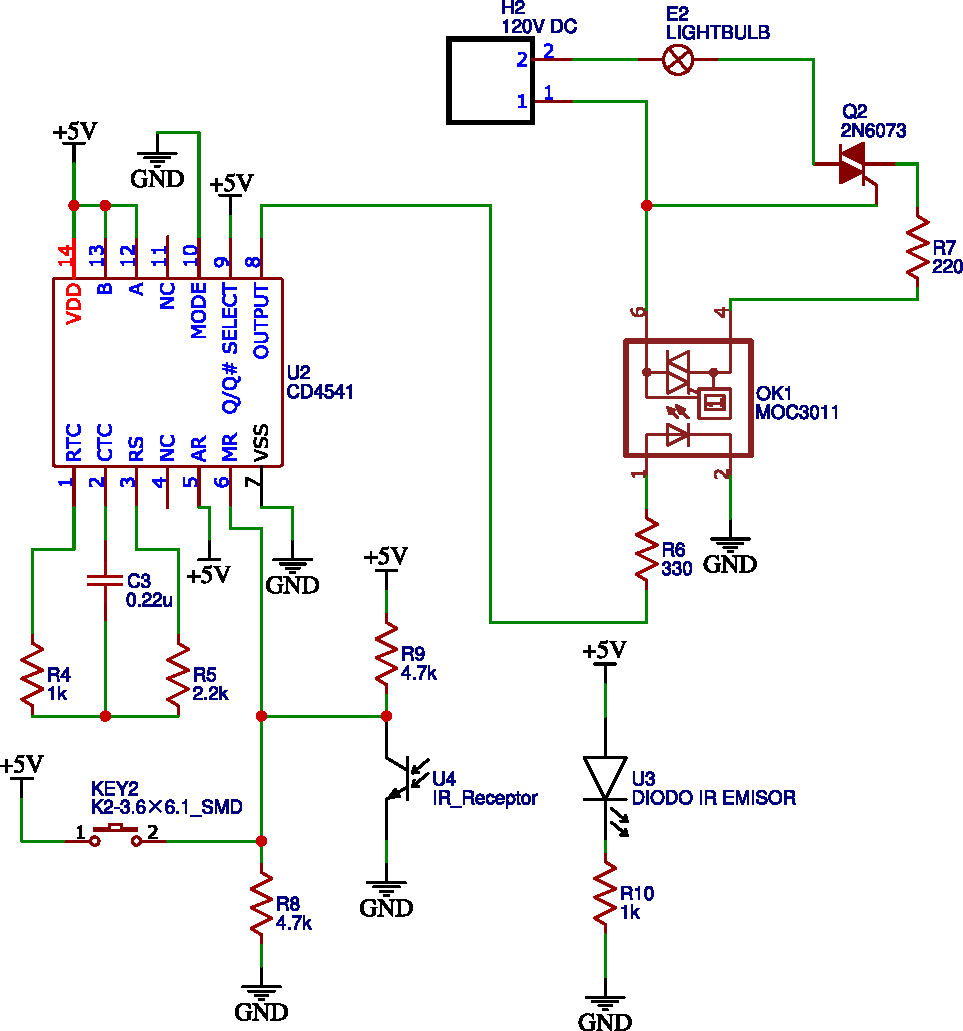
\includegraphics[width=0.8\textwidth]{media/circuito_08}
    \caption{Circuito utilizado en la práctica 8.}
    \label{Fig: Circuito utilizado en la practica 8}
\end{figure}

Para este circuito no tuvimos que realizar ningún cambio de valores ni para voltajes, corrientes ni componentes, ya que logramos conseguir los componentes especificados en la práctica. En la \cref{Fig: Fotografias del circuito realizado durante la practica 8} se puede observar el circuito que realizamos físicamente para esta práctica.

\begin{figure}[htb]
    \centering
    \begin{subfigure}[htb]{0.45\textwidth}
        \centering
        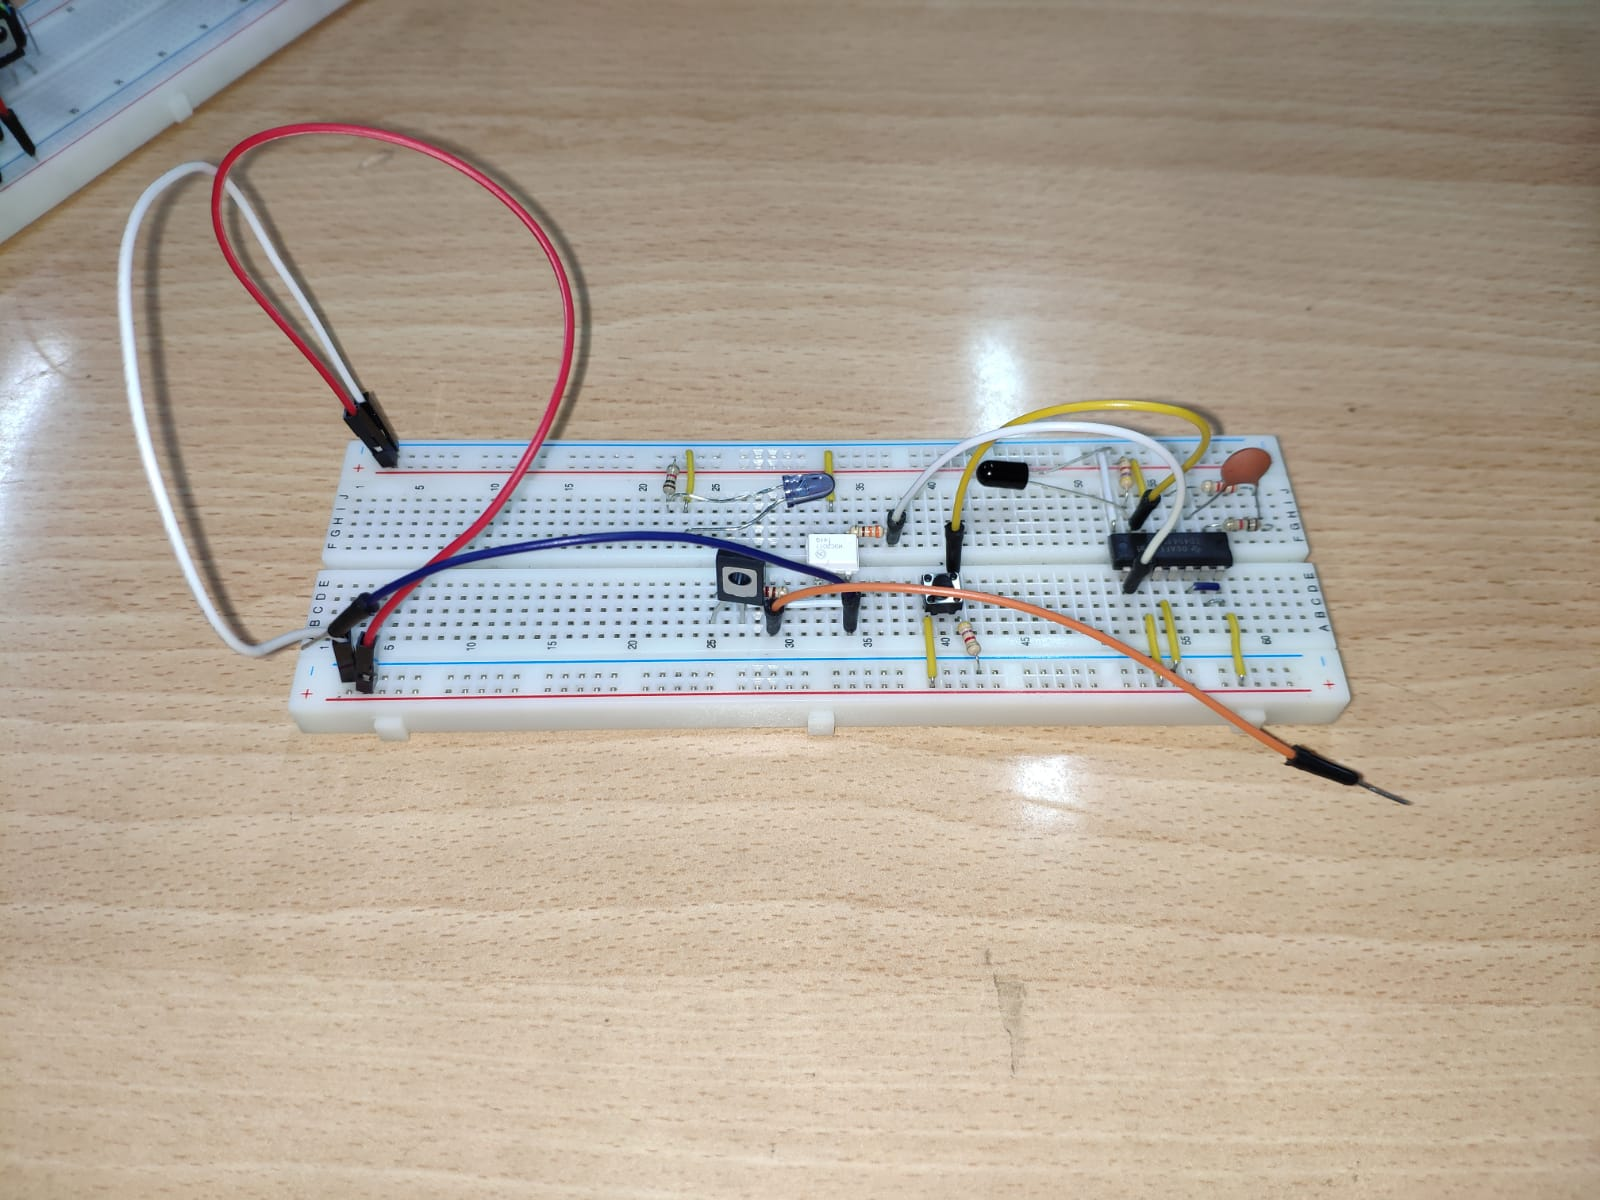
\includegraphics[width=\textwidth]{media/circuito_real_1_08}
        \caption{}
    \end{subfigure}
    \centering
    \begin{subfigure}[htb]{0.45\textwidth}
        \centering
        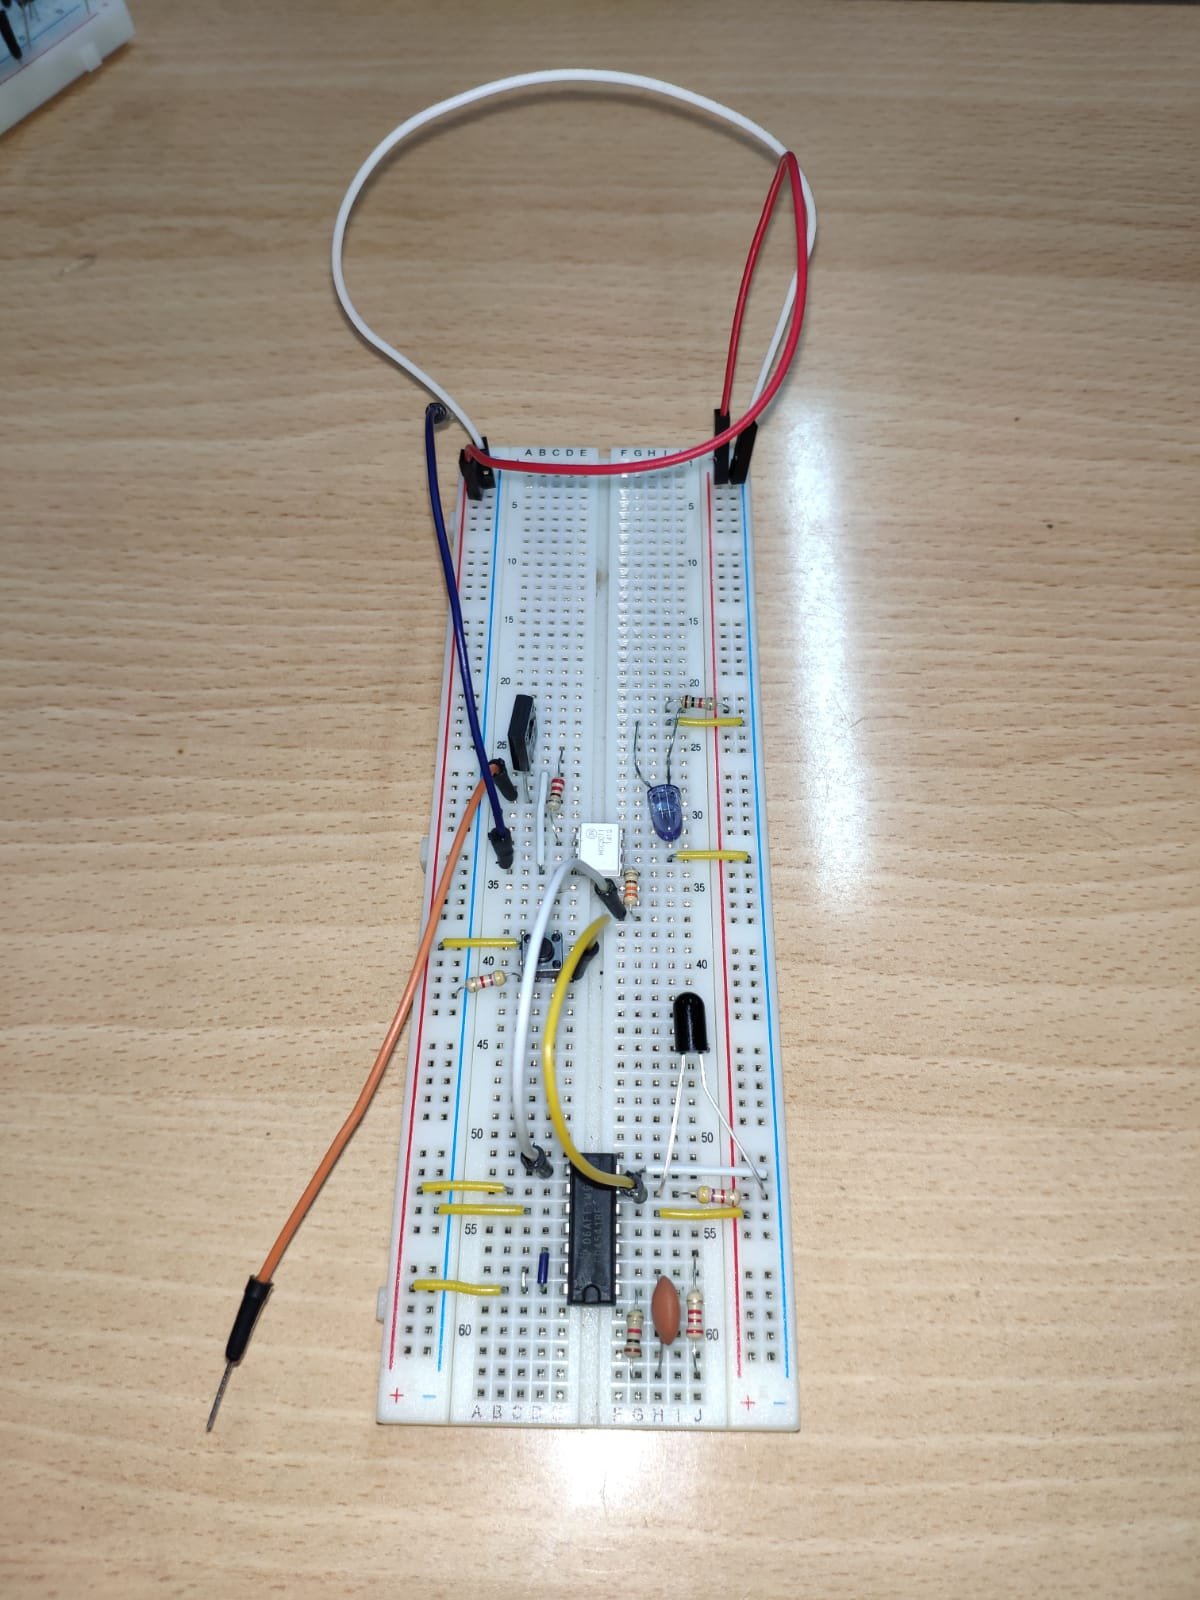
\includegraphics[width=\textwidth]{media/circuito_real_2_08}
        \caption{}
    \end{subfigure}
    \centering
    \begin{subfigure}[htb]{0.45\textwidth}
        \centering
        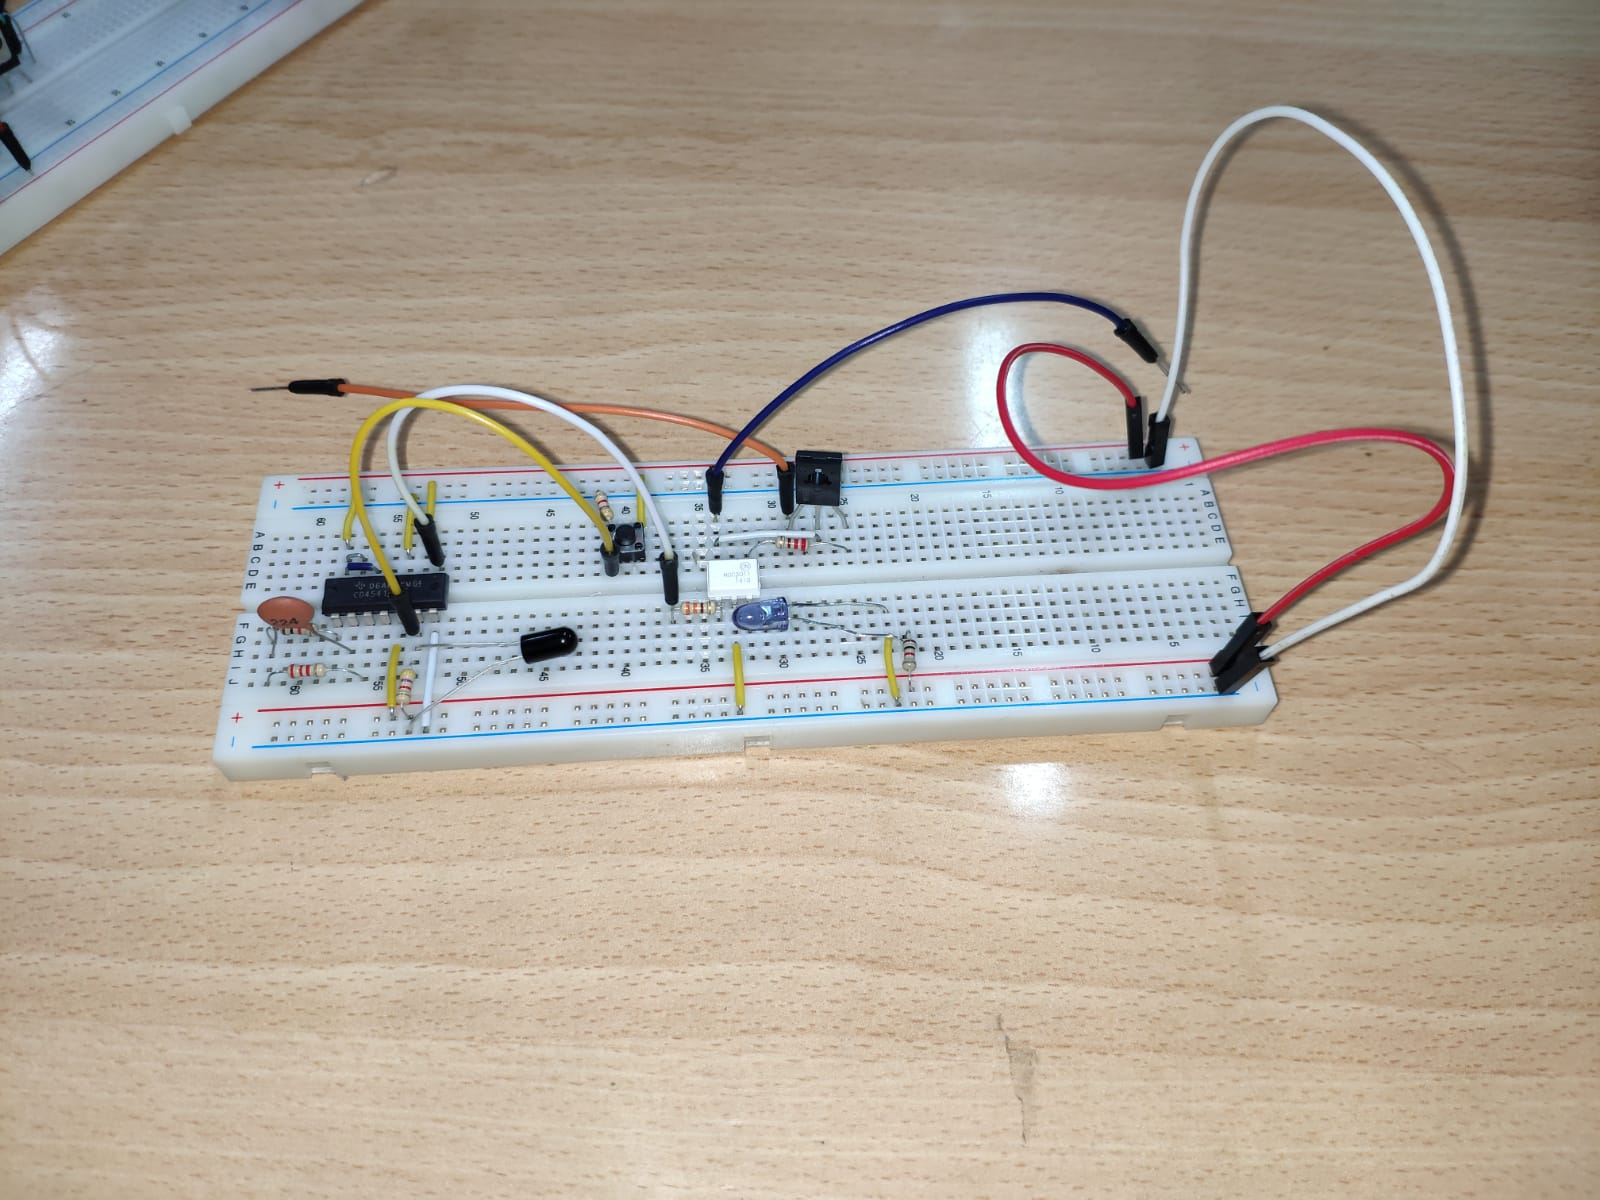
\includegraphics[width=\textwidth]{media/circuito_real_3_08}
        \caption{}
    \end{subfigure}
    \caption{Fotografías del circuito realizado durante la práctica 8.}
    \label{Fig: Fotografias del circuito realizado durante la practica 8}
\end{figure}

\subsection{Resultados}

Debido a que conseguimos todos los elementos sin necesidad de cambiar nigún valor, la práctica funcionó como debería. El único problema que nos encontramos fue con la sensibilidad de la señal entre el receptor y el emisor infrarojo, ya que para poder activar el reset por medio de ese medio, había que poner la mano y cortar la señal en un lugar sumamente específico. Al principio pensamos que estaba mal conectado, pero, al probar con el botón y ver el funcionamiento correcto, nos dimos cuenta que era problema de la sensibilidad del receptor y/o emisor infrorrojo.

\subsection{Conclusiones}

Como se mencionó en la práctica anterior, los timers tienen una gran utilidad en la vida real, especialmente cuando, contrario a la práctica anterior, tienen una etapa de control mucho mejor, que permite al usuario o a la máquina poder toma una segunda decisión después de haber presionar o activado el timer por la primera vez. Esto lo hace una opción más factible para la mayoría de los casos de la vida real, ya que es más flexible con los errores o con las decisiones tardías.

